% !TEX program = pdflatex
% !TEX options = -synctex=1 -interaction=nonstopmode -file-line-error "%DOC%"
% Group Theory Assignment 09
\documentclass[UTF8,10pt,a4paper]{article}
\usepackage[scheme=plain]{ctex}
\newcommand{\CourseName}{Group Theory}
\newcommand{\CourseCode}{PHYS2102}
\newcommand{\Semester}{Spring, 2020}
\newcommand{\ProjectName}{Assignment 09}
\newcommand{\DueTimeType}{Due Time}
\newcommand{\DueTime}{8:15, May 13, 2020 (Wednesday)}
\newcommand{\StudentName}{陈稼霖}
\newcommand{\StudentID}{45875852}
\usepackage[vmargin=1in,hmargin=.5in]{geometry}
\usepackage{fancyhdr}
\usepackage{lastpage}
\usepackage{calc}
\pagestyle{fancy}
\fancyhf{}
\fancyhead[L]{\CourseName}
\fancyhead[C]{\ProjectName}
\fancyhead[R]{\StudentName}
\fancyfoot[R]{\thepage\ / \pageref{LastPage}}
\setlength\headheight{12pt}
\fancypagestyle{FirstPageStyle}{
    \fancyhf{}
    \fancyhead[L]{\CourseName\\
        \CourseCode\\
        \Semester}
    \fancyhead[C]{{\Huge\bfseries\ProjectName}\\
        \DueTimeType\ : \DueTime}
    \fancyhead[R]{Name : \makebox[\widthof{\StudentID}][s]{\StudentName}\\
        Student ID\@ : \StudentID\\
        Score : \underline{\makebox[\widthof{\StudentID}]{}}}
    \fancyfoot[R]{\thepage\ / \pageref{LastPage}}
    \setlength\headheight{36pt}
}
\usepackage{amsmath,amssymb,amsthm,bm}
\allowdisplaybreaks[4]
\newtheoremstyle{Problem}
{}
{}
{}
{}
{\bfseries}
{.}
{ }
{\thmname{#1}\thmnumber{ #2}\thmnote{ (#3)} Score: \underline{\qquad\qquad}}
\theoremstyle{Problem}
\newtheorem{prob}{Problem}
\newtheoremstyle{Solution}
{}
{}
{}
{}
{\bfseries}
{:}
{ }
{\thmname{#1}}
\makeatletter
\def\@endtheorem{\qed\endtrivlist\@endpefalse}
\makeatother
\theoremstyle{Solution}
\newtheorem*{sol}{Solution}
\providecommand{\abs}[1]{\left\lvert#1\right\rvert}
\usepackage{ulem}
\usepackage{graphicx}
\begin{document}
\thispagestyle{FirstPageStyle}
Consider the two-dimensional triangular Bravais lattice (also referred to as the hexagonal Bravais lattice) shown in the figure.
\begin{figure}[h]
    \centering
    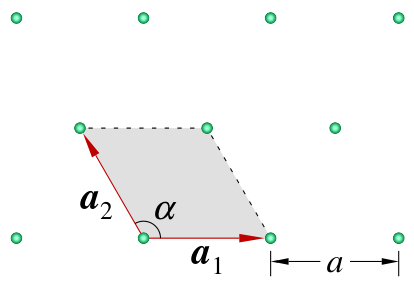
\includegraphics[width=.2\textwidth]{HexagonalBravaisLattice.png}
\end{figure}
\\The basis lattice vectors are given by
\[
    a_1=ae_x,\quad a_2=-(a/2)e_x+(\sqrt{3}/2)e_y.
\]

\begin{prob}
    Find the crystallographic point group of the triangular Bravais lattice. What is the space group of the triangular Bravais lattice in the international system?
\end{prob}
\begin{sol}
    The allowed point symmetry operations of the triangular Bravais lattice are $\{E,C_6,C_6^2=C_3,C_6^3=C_2,C_6^4=C_3^2,C_6^5,C_2^{'(1)},C_2^{'(2)},C_2^{'(3)},C_2^{''(1)},C_2^{''(2)},C_2^{''(3)},I,S_6,S_3,S_3^5,S_6^5,\sigma_h,\sigma_v,\sigma_v',\sigma_v'',\sigma_d,\sigma_d',\sigma_d''\}$, so the crystallographic point group is $\frac{6}{m}mm\,(D_{6h})$.

    The bravais lattice type is primitive lattice ($P$), so the space group of the triangular Bravais lattice in the international system is $P\frac{6}{m}mm$.
\end{sol}

\begin{prob}
    Construct the character table for the crystallographic point group of the triangular Bravais lattice.
\end{prob}
\begin{sol}
    The multiplication table of $D_{6h}$ is so large that I have to omit it here. But I do construct the subgroups and classes of $D_{6h}$. The subgroups of $D_{6h}$ are
    \[
        C_1,C_s,C_i,C_2,C_3,C_6,D_2,D_3,D_6,C_{2v},C_{3v},C_{6v},C_{2h},C_{3h},C_{6h},D_{2h},D_{3h},S_6,D_{6h}.
    \]
    The classes of $D_{6h}$ are
    \[
        \{E\},\quad\{2C_6\},\quad\{2C_3\},\quad\{C_2\},\quad\{3C_2'\},\quad\{3C_2''\},\quad\{I\},\quad\{2S_6\},\quad\{2S_3\},\quad\{\sigma_h\},\quad\{3\sigma_v\},\quad\{3\sigma_d\}.
    \]
    The number of inequivalent irreducible representations is equal to the number of classes of $D_{6h}$, so there are $12$ inequivalent irreducible representations of $D_{6h}$. Suppose the dimension of the $p$th inequivalent irreducible representation of $D_{6h}$ is $d_p$. The sum of the square of the dimensions of the inequivalent irreducible representations of $D_{6h}$ is equal to the order of $D_{6h}$:
    \begin{align}
        \sum_{p=1}^{12}d_p^2=24.
    \end{align}
    Solving the above equation, we get
    \begin{align}
        d_1=d_2=\cdots=d_8=1,\quad d_9=d_{10}=d_{11}=d_{12}=2,
    \end{align}
    so $D_{6h}$ has $8$ inequivalent irreducible representations of order $1$ and $4$ inequivalent irreducible representations of order $2$.\\
    The representation of the identity element is always identity matrix, so its character is equal to the dimension of the representation:
    \begin{align}
        \chi^p(E)=d_p=\left\{\begin{array}{ll}
            1,&p=1,2,\cdots,8,\\
            2,&p=9,10,11,12.
        \end{array}\right.
    \end{align}
    Since $C_2^2=C_2^{'2}=C_2^{''2}=I=\sigma_h^2=\sigma_v^2=\sigma_d^2=E$, we have
    \begin{align}
        \chi^p(\{C_2\})=&\pm 1,\quad p=1,2,\cdots,8,\\
        \chi^p(\{3C_2'\})=&\pm 1,\quad p=1,2,\cdots,8,\\
        \chi^p(\{3C_2''\})=&\pm 1,\quad p=1,2,\cdots,8,\\
        \chi^p(\{I\})=&\pm 1,\quad p=1,2,\cdots,8,\\
        \chi^p(\{\sigma_h\})=&\pm 1,\quad p=1,2,\cdots,8,\\
        \chi^p(\{3\sigma_v\})=&\pm 1,\quad p=1,2,\cdots,8,\\
        \chi^p(\{3\sigma_d\})=&\pm 1,\quad p=1,2,\cdots,8,
    \end{align}
    and thus
    \begin{align}
        \chi^p(\{E\})=1,\quad p=1,2,\cdots,8.
    \end{align}
    The equations above are not all independent:
    \begin{itemize}
        \item Since $C_2\times C_2^{'(1)}=C_2^{''(1)}$, we have
        \begin{align}
            \chi^p(\{C_2\})\chi^p(\{3C_2'\})=\chi^p(\{3C_2''\}),\quad p=1,2,\cdots,8.
        \end{align}
        \item Since $I\times \sigma_h=C_2$, we have
        \begin{align}
            \chi^p(\{I\})\chi^p(\{\sigma_h\})=\chi^p(\{C_2\}),\quad p=1,2,\cdots,8.
        \end{align}
        \item Since $C_2\times\sigma_v=\sigma_d'$, we have
        \begin{align}
            \chi^p(\{C_2\})\chi^p(\{3\sigma_v\})=\chi^p(\{3\sigma_d\}),\quad p=1,2,\cdots,8.
        \end{align}
        \item Since $\sigma_h\times\sigma_v=C_2'$, we have
        \begin{align}
            \chi^p(\{\sigma_h\})\chi^p(\{\sigma_v\})=\chi^p(\{3C_2'\}),\quad p=1,2,\cdots,8.
        \end{align}
    \end{itemize}
    The characters of other classes can be determined by the characters mentioned above
    \begin{itemize}
        \item Since $C_6=C_2^{'(1)}\times C_2^{''(2)}$, we have
        \begin{align}
            \chi^p(\{2C_6\})=\chi^p(\{C_2'\})\chi^p(\{C_2''\}),\quad p=1,2,\cdots,8.
        \end{align}
        \item Since $C_3=C_2^{''(1)}\times C_2^{''(3)}$, we have
        \begin{align}
            \chi^p(\{2C_3\})=\chi^p(\{3C_2''\})\chi^p(\{3C_2''\})=1,\quad p=1,2,\cdots,8.
        \end{align}
        \item Since $S_6=C_6\times\sigma_h$, we have
        \begin{align}
            \chi^p(\{S_6\})=\chi^p(\{2C_6\})\chi^p(\{\sigma_h\}),\quad p=1,2,\cdots,8.
        \end{align}
        \item Since $S_3=C_3\times\sigma_h$, we have
        \begin{align}
            \chi^p(\{S_3\})=\chi^p(\{2C_3\})\chi^p(\{\sigma_h\}),\quad p=1,2,\cdots,8.
        \end{align}
    \end{itemize}
    In this way, for $p=1,2,\cdots,8$, we can determine the characters of all the classes by only knowing $\chi^p(\{C_2\}),\chi^p(\{3C_2'\}),\chi^p(\{I\})$. There are $8$ combinations of $\chi^p(\{C_2\})=\pm 1,\chi^p(\{3C_2'\})=\pm 1,\chi^p(\{I\})=\pm 1$, which correspond to $8$ inequivalent irreducible $1$-dimensional representations.\\
    As for the left four $2$-dimensional inequivalent irreducible representations, we use the orthogonality relation for characters:
    \begin{align}
        \frac{1}{g}\sum_{T\in D_{6h}}\chi^p(T)^*\chi^q(T)=\delta_{pq}
    \end{align}
    for $p=1,2,\cdots,8$ and $q=9,10,11,12$, so
    \tiny
    \begin{align}
        \label{2-1}\chi^q(\{E\})+2\chi^q(\{2C_6\})+2\chi^q(\{2C_3\})+\chi^q(\{C_2\})+3\chi^q(\{3C_2'\})+3\chi^q(\{3C_2''\})+\chi^q(\{I\})+2\chi^q(\{2S_3\})+2\chi^q(\{2S_6\})+\chi^q(\{\sigma_h\})+3\chi^q(\{3\sigma_v\})+3\chi^q(\{3\sigma_d\})=&0,\\
        \label{2-2}\chi^q(\{E\})+2\chi^q(\{2C_6\})+2\chi^q(\{2C_3\})+\chi^q(\{C_2\})+3\chi^q(\{3C_2'\})+3\chi^q(\{3C_2''\})-\chi^q(\{I\})-2\chi^q(\{2S_3\})-2\chi^q(\{2S_6\})-\chi^q(\{\sigma_h\})-3\chi^q(\{3\sigma_v\})-3\chi^q(\{3\sigma_d\})=&0,\\
        \label{2-3}\chi^q(\{E\})+2\chi^q(\{2C_6\})+2\chi^q(\{2C_3\})+\chi^q(\{C_2\})-3\chi^q(\{3C_2'\})-3\chi^q(\{3C_2''\})+\chi^q(\{I\})+2\chi^q(\{2S_3\})+2\chi^q(\{2S_6\})+\chi^q(\{\sigma_h\})-3\chi^q(\{3\sigma_v\})-3\chi^q(\{3\sigma_d\})=&0,\\
        \label{2-4}\chi^q(\{E\})+2\chi^q(\{2C_6\})+2\chi^q(\{2C_3\})+\chi^q(\{C_2\})-3\chi^q(\{3C_2'\})-3\chi^q(\{3C_2''\})-\chi^q(\{I\})-2\chi^q(\{2S_3\})-2\chi^q(\{2S_6\})-\chi^q(\{\sigma_h\})+3\chi^q(\{3\sigma_v\})+3\chi^q(\{3\sigma_d\})=&0,\\
        \label{2-5}\chi^q(\{E\})-2\chi^q(\{2C_6\})+2\chi^q(\{2C_3\})-\chi^q(\{C_2\})+3\chi^q(\{3C_2'\})-3\chi^q(\{3C_2''\})+\chi^q(\{I\})-2\chi^q(\{2S_3\})+2\chi^q(\{2S_6\})-\chi^q(\{\sigma_h\})-3\chi^q(\{3\sigma_v\})+3\chi^q(\{3\sigma_d\})=&0,\\
        \label{2-6}\chi^q(\{E\})-2\chi^q(\{2C_6\})+2\chi^q(\{2C_3\})-\chi^q(\{C_2\})+3\chi^q(\{3C_2'\})-3\chi^q(\{3C_2''\})-\chi^q(\{I\})+2\chi^q(\{2S_3\})-2\chi^q(\{2S_6\})+\chi^q(\{\sigma_h\})+3\chi^q(\{3\sigma_v\})-3\chi^q(\{3\sigma_d\})=&0,\\
        \label{2-7}\chi^q(\{E\})-2\chi^q(\{2C_6\})+2\chi^q(\{2C_3\})-\chi^q(\{C_2\})-3\chi^q(\{3C_2'\})+3\chi^q(\{3C_2''\})+\chi^q(\{I\})+2\chi^q(\{2S_3\})-2\chi^q(\{2S_6\})+\chi^q(\{\sigma_h\})-3\chi^q(\{3\sigma_v\})+3\chi^q(\{3\sigma_d\})=&0,\\
        \label{2-8}\chi^q(\{E\})-2\chi^q(\{2C_6\})+2\chi^q(\{2C_3\})-\chi^q(\{C_2\})-3\chi^q(\{3C_2'\})+3\chi^q(\{3C_2''\})-\chi^q(\{I\})-2\chi^q(\{2S_3\})+2\chi^q(\{2S_6\})-\chi^q(\{\sigma_h\})+3\chi^q(\{3\sigma_v\})-3\chi^q(\{3\sigma_d\})=&0,
    \end{align}
    and
    \begin{align}
        \nonumber\abs{\chi^q(\{E\})}^2+2\abs{\chi^q(\{2C_6\})}^2+2\abs{\chi^q(\{2C_3\})}^2+\abs{\chi^q(\{C_2\})}^2+3\abs{\chi^q(\{3C_2'\})}^2+3\abs{\chi^q(\{3C_2''\})}^2+\abs{\chi^q(\{I\})}+2\abs{\chi^q(\{2S_3\})}^2+2\abs{\chi^q(\{2S_6\})}^2&\\
        \label{2-9}+\abs{\chi^q(\{\sigma_h\})}^2+3\abs{\chi^q(\{3\sigma_v\})}^2+3\abs{\chi^q(\{3\sigma_d\})}^2&=24,
    \end{align}
    \normalsize
    for $q=9,10,11,12$. We already know that the character of the identity element is always equal to the dimension of the representation, $\chi^q(\{E\})=2$ for $q=9,10,11,12$. Adding the equation \eqref{2-1}$\sim$\eqref{2-8}, we get
    \begin{align}
        \chi^q(\{E\})+2\chi^q(\{2C_3\})=0,\quad q=9,10,11,12,
    \end{align}
    so
    \begin{align}
        \chi^q(\{2C_3\})=-1,\quad q=9,10,11,12.
    \end{align}
    Adding equations \eqref{2-1}$\sim$\eqref{2-4}, we get
    \begin{align}
        \chi^q(\{E\})+2\chi^q(\{2C_6\})+2\chi^q(\{2C_3\})+\chi^q(\{C_2\})=0,\quad q=9,10,11,12,
    \end{align}
    so
    \begin{align}
        2\chi^q(\{2C_6\}+\chi^q(\{C_2\})=0,\quad q=9,10,11,12.
    \end{align}
    Adding equations \eqref{2-1} and \eqref{2-2}, we get
    \begin{align}
        \chi^q(\{E\})+2\chi^q(\{2C_6\})+2\chi^q(\{2C_3\})+\chi^q(\{C_2\})+3\chi^q(\{3C_2'\})+3\chi^q(\{3C_2''\})=0,\quad q=9,10,11,12,
    \end{align}
    so
    \begin{align}
        \chi^q(\{3C_2'\})+\chi^q(\{3C_2''\})=0,\quad q=9,10,11,12
    \end{align}
    Adding equation \eqref{2-1}, \eqref{2-2}, \eqref{2-5} and \eqref{2-6}, we get
    \begin{align}
        \chi^q(\{E\})+2\chi^q(\{2C_3\})+3\chi^q(\{3C_2'\})=0,\quad q=9,10,11,12,
    \end{align}
    so
    \begin{align}
        \chi^q(\{3C_2'\})=0,\quad q=9,10,11,12,
    \end{align}
    and
    \begin{align}
        \chi^q(\{3C_2''\})=0,\quad q=9,10,11,12.
    \end{align}
    Adding equations \eqref{2-1} and \eqref{2-4}, we get
    \begin{align}
        \chi^q(\{E\})+2\chi^q(\{2C_6\})+2\chi^q(\{2C_3\})+\chi^q(\{C_2\})+3\chi^q(\{3\sigma_v\})+3\chi^q(\{3\sigma_d\})=0,\quad q=9,10,11,12,
    \end{align}
    so
    \begin{align}
        \chi^q(\{3\sigma_v\})+\chi^q(\{3\sigma_d\})=0,\quad q=9,10,11,12.
    \end{align}
    Subtracting \eqref{2-1} from \eqref{2-2}, we get
    \begin{align}
        \chi^q(\{I\})+2\chi^q(\{2S_3\})+2\chi^q(\{2S_6\})+\chi^q(\{\sigma_h\})+3\chi^q(\{3\sigma_v\})+3\chi^q(\{3\sigma_d\})=0,\quad q=9,10,11,12,
    \end{align}
    so
    \begin{align}
        \chi^q(\{I\})+2\chi^q(\{2S_3\})+2\chi^q(\{2S_6\})+\chi^q(\{\sigma_h\})=0,\quad q=9,10,11,12.
    \end{align}
    $\cdots$ There $48$ unknown characters for $q=9,10,11,12$, and $42$ equations from the orthogonality relation for characters plus the fact that $\chi^q(\{E\})=2$ for $q=9,10,11,12$, technically, we may obtain all the characters for the four $2$-dimensional inequivalent irreducible representations. $\cdots$\\
    The character table of $D_{6h}$ is shown in table \ref{CT}.
    \newpage
    \begin{table}[h]
        \centering
        \caption{The character table of $D_{6h}$.}
        \label{CT}
        \begin{tabular}{c|cccccccccccc}
            & $\{E\}$ & $\{2C_6\}$ & $\{2C_3\}$ & $\{C_2\}$ & $\{3C_2'\}$ & $\{3C_2''\}$ & $\{I\}$ & $\{2S_3\}$ & $\{2S_6\}$ & $\{\sigma_h\}$ & $\{3\sigma_v\}$ & $\{3\sigma_d\}$ \\ \hline
           $\Gamma^1$ & $1$ & $1$ & $1$ & $1$ & $1$ & $1$ & $1$ & $1$ & $1$ & $1$ & $1$ & $1$ \\
           $\Gamma^2$ & $1$ & $1$ & $1$ & $1$ & $1$ & $1$ & $-1$ & $-1$ & $-1$ & $-1$ & $-1$ & $-1$ \\
           $\Gamma^3$ & $1$ & $1$ & $1$ & $1$ & $-1$ & $-1$ & $1$ & $1$ & $1$ & $1$ & $-1$ & $-1$ \\
           $\Gamma^4$ & $1$ & $1$ & $1$ & $1$ & $-1$ & $-1$ & $-1$ & $-1$ & $-1$ & $-1$ & $1$ & $1$ \\
           $\Gamma^5$ & $1$ & $-1$ & $1$ & $-1$ & $1$ & $-1$ & $1$ & $-1$ & $1$ & $-1$ & $-1$ & $1$ \\
           $\Gamma^6$ & $1$ & $-1$ & $1$ & $-1$ & $1$ & $-1$ & $-1$ & $1$ & $-1$ & $1$ & $1$ & $-1$ \\
           $\Gamma^7$ & $1$ & $-1$ & $1$ & $-1$ & $-1$ & $1$ & $1$ & $1$ & $-1$ & $1$ & $-1$ & $1$ \\
           $\Gamma^8$ & $1$ & $-1$ & $1$ & $-1$ & $-1$ & $1$ & $-1$ & $-1$ & $1$ & $-1$ & $1$ & $-1$ \\
           $\Gamma^9$ & $2$ & $1$ & $-1$ & $-2$ & $0$ & $0$ & $2$ & $1$ & $-1$ & $-2$ & $0$ & $0$ \\
           $\Gamma^{10}$ & $2$ & $-1$ & $-1$ & $2$ & $0$ & $0$ & $2$ & $-1$ & $-1$ & $2$ & $0$ & $0$ \\
           $\Gamma^{11}$ & $2$ & $1$ & $-1$ & $-2$ & $0$ & $0$ & $-2$ & $-1$ & $1$ & $2$ & $0$ & $0$ \\
           $\Gamma^{12}$ & $2$ & $-1$ & $-1$ & $2$ & $0$ & $0$ & $-2$ & $1$ & $1$ & $-2$ & $0$ & $0$
        \end{tabular}
    \end{table}
\end{sol}

\begin{prob}
    Find the basis lattice vectors of the reciprocal lattice of the triangular Bravais lattice. Show that the first Brillouin zone of the triangular Bravais lattice is as given in the following figure.
    \begin{figure}[h]
        \centering
        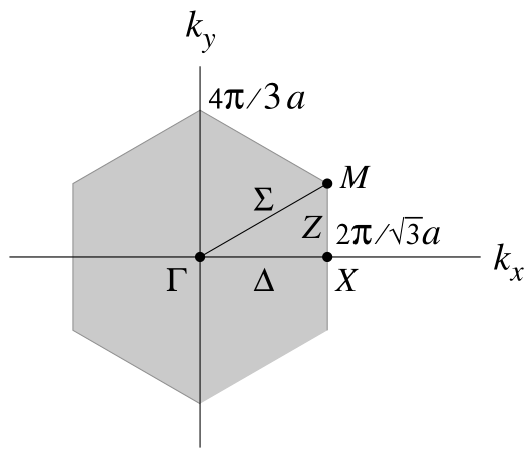
\includegraphics[width=.2\textwidth]{FirstBrillouinZone.png}
    \end{figure}
\end{prob}
\begin{sol}
    The basis lattice vectors of the reciprocal lattice of the triangular Bravais lattice are
    \begin{align}
        \bm{b}_1=&\frac{2\pi\bm{a}_2\times\hat{e}_z}{\hat{e}_z\cdot(\bm{a}_1\times\bm{a}_2)}=\frac{4\pi}{\sqrt{3}a}(\frac{\sqrt{3}}{2}\hat{e}_x+\frac{1}{2}\hat{e}_y),\\
        \bm{b}_2=&\frac{2\pi\hat{e}_z\times\bm{a}_1}{\hat{e}_z\cdot(\bm{a}_1\times\bm{a}_2)}=\frac{4\pi}{\sqrt{3}a}\hat{e}_y.
    \end{align}
    As shown in figure \ref{3-RLFB}, we construct the reciprocal lattice of the triangular Bravais. We join the original point $\vec{k}=0$ of the reciprocal lattice and the six nearest reciprocal lattice points around it with \dashuline{dash line}. We draw the perpendicular bisectors of these lines with \dotuline{dotty line}. The region enclosed by these \dotuline{dotty line} is the first Brillouin region, which is the same as figure given above.
    \newpage
    \begin{figure}[h]
        \centering
        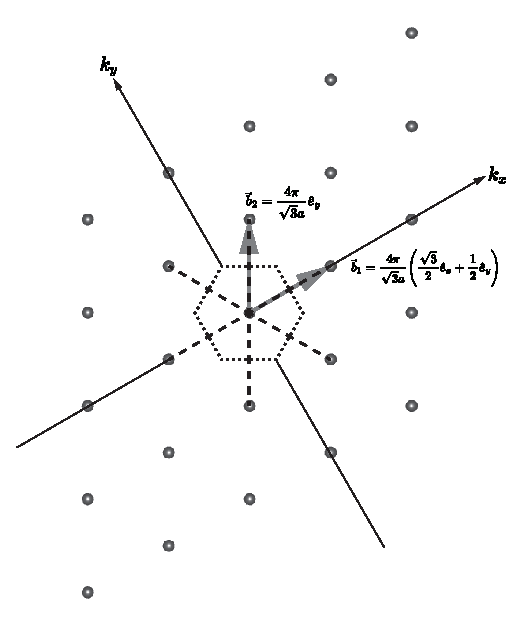
\includegraphics[width=.4\textwidth]{3.eps}
        \caption{The reciprocal lattice and the first Brillouin of triangular Bravais lattice.}
        \label{3-RLFB}
    \end{figure}
\end{sol}

\begin{prob}
    Find the point groups for the $\vec{k}$-vectors: $\vec{k}_{\Gamma}=\vec{0}$, $\vec{k}_X$, and $\vec{k}_M$.
\end{prob}
\begin{sol}
    $\vec{k}_{\Gamma}$ remains invariant under all the point symmetry operations of $D_{6h}$, so the point groups for $\vec{k}_{\Gamma}$ is $D_{6h}$.\\
    $\vec{k}_X$ remains invariant under the point symmetry operations $\{E,C_2,C_2',C_2'',I,\sigma_h,\sigma_v,\sigma_d\}$, so the point group for $\vec{k}_X$ is $D_{2h}$.\\
    $\vec{k}_M$ remains invariant under the point symmetry operations $\{E,C_3,C_3^2,C_2',C_2'',C_2''',S_3,S_3^5,\sigma_h,\sigma_v,\sigma_v',\sigma_v''\}$, so the point group for $\vec{k}_M$ is $D_{3h}$.
\end{sol}

\begin{prob}
    Identify the symmetry axes and their point groups in the first Brillouin zone of the triangular Bravais lattice.
\end{prob}
\begin{sol}
    The symmetry axes in the first Brillouin zone of the triangular Bravais lattice is shown in figure \ref{5-FBSA}.
    \begin{figure}[h]
        \centering
        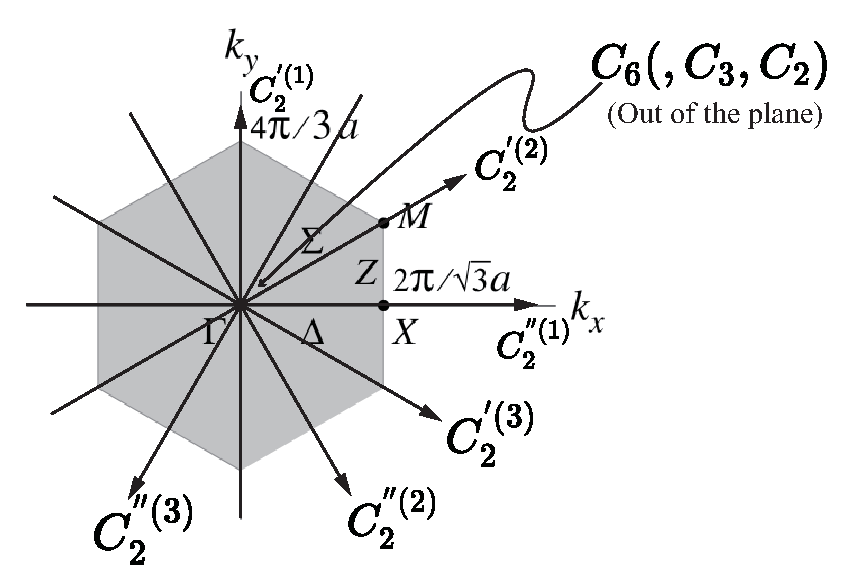
\includegraphics[width=.45\textwidth]{5-Gamma.eps}
        \caption{The first Brillouin zone and the symmetry axes.}
        \label{5-FBSA}
    \end{figure}
    \\The $C_2^{'(j)}$ and $C_2^{''(j)}$ axes ($j=1,2,3$) remain invariant under the point symmetry operations $\{E,I,C_2,C_2',C_2'',\sigma_h,\sigma_v,\sigma_v'\}$, so the point group of the $C_2^{'(j)}$ and $C_2^{''(j)}$ axes ($j=1,2,3$) are all $D_{2h}$.\\
    The $C_6$ axis remains invariant under all the point symmetry operations of $D_{6h}$, so the point group of the $C_6$ axis is $D_{6h}$.
\end{sol}
\end{document}